\section{Introduction}
Model reference control allows the user to design a controller without the need to estimate a parametric model of the open loop system. However, the stability of the closed loop system is not guaranteed when minimizing (\ref{eq:Jmr}) or (\ref{eq:J}). If a parametric representation of the TF of an LTI system is known, then the stability of the closed loop system can be inferred by analysing the poles of the closed loop system. As long as none of the poles are in the right half plane of the complex plane for CT systems, then the closed loop system is stable. To ensure the stability for DT system, none of the poles are allowed to be outside of the unit circle in the complex plane. In data-driven model reference control, the locations of the poles are unknown, which means we must find another way to guarantee the stability of the closed loop system. The following is a detailed repetition of the idea presented in \cite{Data-driven_model_reference_control}. We will first give a small explanation of the small-gain theorem and will then show how this theorem can be used to guarantee the stability in data-driven model reference control. 
%Finally, this stability constraint will be used to design an analog controller for a real system.

\section{Small-gain theorem}
The small-gain theorem can be seen as a generalization of the Nyquist criterion to nonlinear time-varying system \cite{Zames1966}. Assume that we have an interconnection of 2 stable LTI systems as shown in figure \ref{fig:interconnection}.

\begin{figure}[H]
\centering
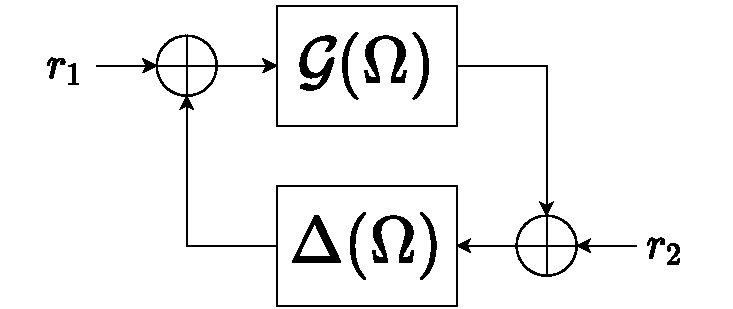
\includegraphics[width = 0.45\textwidth]{figures/interconnection.pdf}
\caption{An interconnection of 2 stable LTI systems.}
\label{fig:interconnection}
\end{figure}

A specific case of the small-gain theorem \cite{control_theory_ljung} states that the interconnection of these two stable LTI systems is stable if 
\begin{equation}
||\mathcal{G}(\Omega)\Delta(\Omega)||_\infty < 1
\end{equation}
with $||\bullet||$ being the H-infinity norm of an LTI system defined as
\begin{equation*}
	||H(\Omega)||_\infty = \begin{cases}
		\sup_\omega |H(j\omega)| & \text{for CT systems} \\
		\sup_\omega |H(e^{j\omega})| & \text{for DT systems} \\
	\end{cases}
\end{equation*}

\paragraph{Example}
Consider a simple example of a CT system being controlled with a proportional controller in negative feedback. 
\begin{align*}
\mathcal{G}(s) &= \frac{1}{s+2}\\
\Delta(s) &= K_P
\end{align*}
Then
\begin{equation}
|\mathcal{G}(j\omega)\Delta(j\omega)|^2 = \Big|\frac{1}{j\omega+2}K_P\Big|^2 = \frac{K_P^2}{\omega^2 + 4}
\label{eq:GDeltasquared}
\end{equation}
The quantity (\ref{eq:GDeltasquared}) must be smaller than 1 for all $\omega \in \mathds{R}$.
\begin{align*}
\Rightarrow &K_P^2 < \omega^2 + 4 \quad \forall \omega \in \mathds{R} \\
\Leftrightarrow  & K_P^2-4 < \omega^2 \quad \forall \omega \in \mathds{R}
\end{align*}
If the above inequality holds for $\omega = 0$, then the above inequality holds for all $\omega \in \mathds{R}$.
\begin{equation}
K_P^2-4 < 0 \Rightarrow \boxed{-2 < K_P < 2}
\label{eq:Kpboundssmallgain}
\end{equation}

According to the small-gain theorem, choosing $K_P$ between -2 and 2 will guarantee the stability of the closed loop system. Let's now compare this result to the traditional way of determining whether the closed loop system is stable: by analysing the location of the closed loop poles. The closed loop system is given by
\begin{equation*}
	\frac{\mathcal{G}(s)}{1 + \mathcal{G}(s)\Delta(s)} = \frac{\frac{1}{s+2}}{1 + \frac{K_P}{s+2}} = \frac{1}{s + 2 + K_P}
\end{equation*}
The location of the closed loop pole is $-(2+K_P)$. To ensure stability, the real part of the pole must be smaller than 0
\begin{equation}
-(2 + K_P) < 0 \Rightarrow \boxed{-2 < K_P}
\label{eq:Kpboundstradition}
\end{equation}
The bounds (\ref{eq:Kpboundssmallgain}) are contained in the bounds (\ref{eq:Kpboundstradition}). Thus, we can conclude that the stability bounds given by the small-gain theorem are much more conservative. For example, choosing $K_P=4$ will still result in a stable closed loop system. The nice thing about the small-gain theorem, is that it is sufficient to have a nonparametric estimate of the FRF of $\mathcal{G}(\Omega)$ and $\Delta(\Omega)$ in order to determine whether the closed loop system will be stable. Contrast this with the need to know the location of the poles of $\mathcal{G}(\Omega)$ to get to (\ref{eq:Kpboundstradition}).

\subsection{Stability constraints}
\label{sec:stability_constraints}
In data-driven model reference control, the user does not have access to a parametric representation of the TF of the system $G(\Omega)$. However, we can estimate the FRF of the system nonparametrically. This nonparametric estimate can be used to guarantee stability by using the small-gain theorem.

Looking back at figure \ref{fig:closed_loop_system}, we can see that $\mathcal{G}(\Omega) = K(\Omega,\rho) G(\Omega)$, $\Delta = 1$, $r_1 = r - v$ and $r_2 = 0$. In order to use the small-gain theorem, $\mathcal{G}$ and $\Delta$ must be stable. As $K(\Omega,\rho)$ is stable by construction, this means that $G(\Omega)$ must be stable. Thus, the stability cannot be guaranteed when $G(\Omega)$ is unstable. If $G(\Omega)$ is stable, then the closed loop system is stable if
\begin{equation*}
||K(\Omega,\rho) G(\Omega)||_\infty < 1
\end{equation*}
The problem with this constraint is that it cannot be realized in practice. The quantity $|K(\Omega,\rho) G(\Omega)|$ must be smaller than 1 for all frequencies. In reality, a nonparametric estimate has a certain frequency resolution $f_s/N$, with $f_s$ being the sampling frequency and $N$ being the number of samples in 1 period of the excitation signal. Thus, the user must ensure that the frequency resolution is high enough to not miss any resonance peaks in the FRF. With this in mind, the constraint turns into
\begin{equation*}
|K(\Omega_k,\rho) \hat{G}(\Omega_k)| < 1 \,, \quad \forall k \in \kexc
\end{equation*}
with $\hat{G}(\Omega_k)$ being the estimate of the FRF of $G(\Omega)$ at the $k$-th DFT bin and $\kexc$ being the set of excited harmonics.

The optimization can then be done in the following way:
\begin{align*}
	&\hat{\rho} = \underset{\rho}{\mathrm{arg\,min}} \, J(\rho) \\
	\text{subject to } &|K(\Omega_k,\rho) \hat{G}(\Omega_k)| < 1 \quad \forall k \in \kexc
\end{align*}
with $J(\rho)$ being the TD cost function (\ref{eq:JNl1}), FD cost function (\ref{eq:JFD}) or the FD cost function with $l_1$-trick (\ref{eq:JNl1_FD}). As the cost function is a convex function and the constraints are convex, the optimization problem as a whole is also convex, meaning that it can be solved with a convex solver.

\subsection{Better stability constraints}
The stability constraints discussed in the previous section are very conservative. We can do better. The closed loop system that is shown in figure \ref{fig:closed_loop_system} can be redrawn as shown in figure \ref{fig:small_gain_CL1}. The reference signal $r$ was grouped together with the output noise $v$ and the controller was split up into 2 branches by using $K(\rho) = (K(\rho) - K^*) + K^*$, with $K^*$ being the ideal controller that might not be realizable by the proposed controller structure $K(\rho)$.

\begin{figure}[H]
\centering
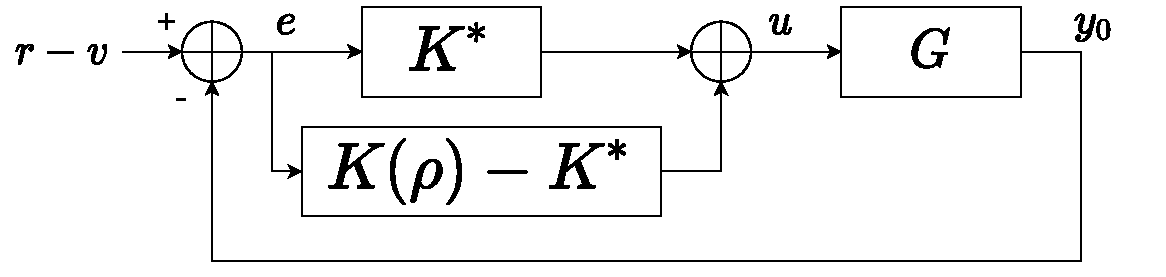
\includegraphics[scale=0.6]{figures/small_gain_CL1}
\caption{Redrawing figure \ref{fig:closed_loop_system} by using $K(\rho) = (K(\rho) - K^*) + K^*$ and by grouping the reference $r$ with the output noise $v$.}
\label{fig:small_gain_CL1}
\end{figure}

The next step involves shifting the system $G(\Omega)$ into the 2 newly created branches. This is shown in figure \ref{fig:small_gain_CL2}.
 
\begin{figure}[H]
\centering
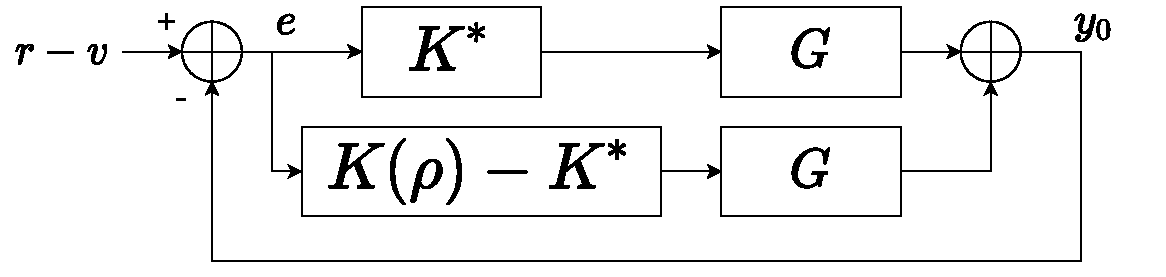
\includegraphics[scale=0.6]{figures/small_gain_CL2}
\caption{Redrawing figure \ref{fig:small_gain_CL1} by shifting $G(\Omega)$ to the left.}
\label{fig:small_gain_CL2}
\end{figure}

Finally, by playing around with the summations we arrive at the block diagram shown in figure \ref{fig:small_gain_CL3}.
\begin{figure}[H]
\centering
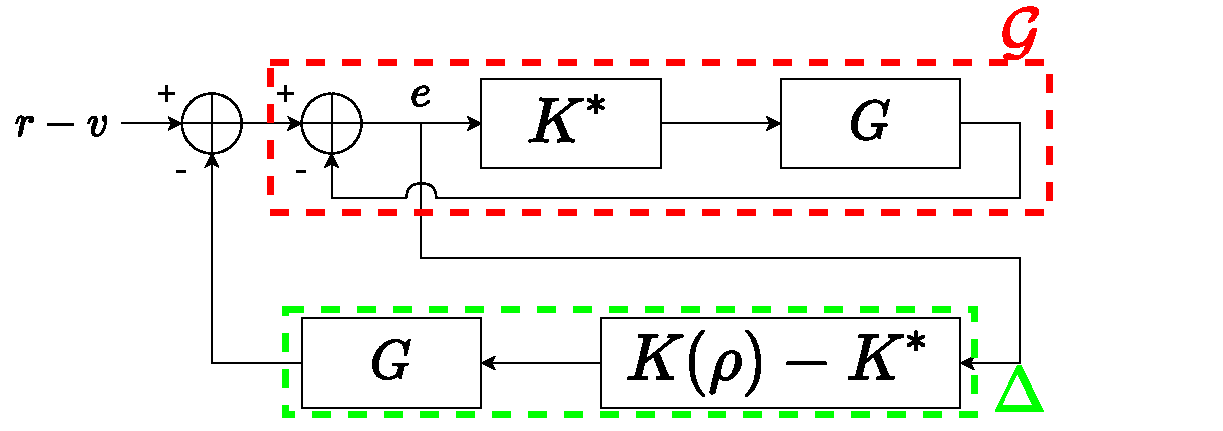
\includegraphics[scale=0.6]{figures/small_gain_CL3}
\caption{Redrawing figure \ref{fig:small_gain_CL2} by playing around with the summations.}
\label{fig:small_gain_CL3}
\end{figure}


With a little bit of imagination, we can see that this is an interconnection of 2 systems.
\begin{align*}
\mathcal{G} &= \frac{1}{1+K^*G} = 1-M\\
\Delta &= (K(\rho)-K^*)G
\end{align*}
The system $\mathcal{G}$ is the TF between the output of the first summer and $e$. To use the small-gain theorem, both $\mathcal{G}$ and $\Delta$ must be stable systems. $\mathcal{G}$ is stable because $M$ is stable by construction. Showing that $\Delta$ is stable is a bit more involved. This is because $K^*$ is not necessarily stable and causal. Using
\begin{equation*}
K^* = \frac{M}{G(1-M)}
\end{equation*}
we can expand $\Delta$
\begin{equation*}
\Delta = K(\rho) G - \frac{M}{G(1-M)} G = K(\rho) G - \frac{M}{1-M}
\end{equation*}
The first term $K(\rho) G$ is stable because $K(\rho)$ is stable by construction and because $G$ is also assumed to be stable. If $G$ is not stable, then the small-gain theorem cannot be used. The second term is not necessarily stable $\frac{M}{1-M}$. However, it can be chosen by the user in such a way that it is stable. The fact that $\frac{M}{1-M}$ must be stable is not mentioned in \cite[Lemma 1]{Data-driven_model_reference_control}. 

Finally, if $\mathcal{G}$ and $\Delta$ are stable, the small-gain theorem says that the stability of the closed loop system is guaranteed if
\begin{align*}
&||\mathcal{G}\Delta||_\infty < 1 \\
\Leftrightarrow & \Big|\Big|(1-M) \big(K(\rho) G - \frac{M}{1-M}\big)\Big|\Big|_\infty < 1 \\
\Leftrightarrow & ||(1-M)K(\rho)G - M||_\infty < 1\\
\Leftrightarrow & ||M -(1-M)K(\rho)G ||_\infty < 1
\end{align*}

The optimization can then be done with these constraints
\begin{align*}
	&\hat{\rho} = \underset{\rho}{\mathrm{arg\,min}} \, J(\rho) \\
	\text{subject to } &|M(\Omega_k) -(1-M(\Omega_k))K(\Omega_k,\rho)\hat{G}(\Omega_k)| < 1 \,, \quad \forall k \in \kexc
\end{align*}
Again, the same rules apply here: the frequency resolution $f_s/N$ must be high enough to not miss any resonance peaks. $J(\rho)$ can be one of the cost function mentioned in section \ref{sec:stability_constraints}. These constraints are also convex, which makes the optimization problem convex. Thus, it can be solved with a convex solver.

These constraints are less conservative than the constraints from section \ref{sec:stability_constraints} for the following reason. If $\hat G$ is replaced by the exact system $G$ and if $K(\rho)$ is replaced by the ideal controller $K^*$ then
\begin{equation*}
M -(1-M)K^*G = M - (1-M)\frac{M}{1-M} = 0
\end{equation*}
which means that the constraints are fulfilled. Thus, $M -(1-M)K(\rho)G$ is a measure of how close the closed loop system is to the stable reference model. This is also evident by noticing that $M -(1-M)K(\rho)G$ is contained inside the convex cost function.
\begin{equation*}
    J(\rho) =  \Big|\Big|F(1-M)) \Big[M-(1-M)K(\rho) G\Big]  \Big|\Big|_2^2 
\end{equation*}

%\section{Conclusion}
%The small-gain theorem was used to derive convex constraints that guarantee the stability of the closed loop system under certain conditions. The FD method was used to design an analog controller for a Wiener-Hammerstein system. The stability constraints were used to guarantee the stability of the closed loop system. Then, the analog controller was constructed successfully. Finally, the analog controller and closed loop system were measured. However, the measurement of the analog controller was not successful. The cause of this failure is unknown.